% !TEX root = DauceAlbigesPerrinet2020.tex
% !TEX encoding = UTF-8 Unicode
% -*- coding: UTF-8; -*-
% vim: set fenc=utf-8
% !TEX spellcheck = en-US
\section{Introduction}
\label{sec:intro}
\subsection{Problem statement}
%------------------------------%
The field of computer vision was recently recast by the outstanding capability of convolution-based deep neural networks to capture the semantic content of images and photographs. Human performance is now outreached by computer algorithms in numerous image categorization tasks~\cite{He15}. One of the reasons explaining this breakthrough is a strong reduction in the number of parameters used to train the network, through a massive sharing of weights in the convolutional layers. Reducing the number of parameters and/or the size of the visual data that needs to be processed is a decisive factor for further improvements. Initially trained on energy greedy, high-performance computers, these algorithms are now designed to work on more common hardware such as desktop computers with dedicated GPU hardware~\cite{Sandler18}. Despite lots of efforts both in hardware and software optimization, the processing of pixel-based images is still done at a cost that scales linearly with the image size: All pixels present in the image are systematically processed by the computer algorithm, even the ones that are useless for the task at hand. Current computer vision algorithms consequently manipulate millions of pixels and millions of variables with ensuing energy consumption, even in the case of downsampled images, and with a still prohibitive cost for large images and videos. The need to detect visual objects at a glance while running on resource-constrained embedded hardware, for instance in autonomous driving, introduces a necessary trade-off between efficiency and accuracy,
requiring renewed mathematical treatment and computational implementations.

Interestingly, things work differently when human vision is considered. First, human vision is still unsurpassable in the case of ecological real-time sensory flows. Indeed, object recognition can be achieved by the human visual system both rapidly, --~in less than $100~\ms$~\cite{Kirchner06}~-- and at a low energy cost ($<5~W$). On top of that, it is mostly self-organized, robust to visual transforms or lighting conditions and can learn with few examples. If many different anatomical features may explain this efficiency, the main difference lies in the fact that its sensor (the retina) combines a non-homogeneous sampling of the world with the capacity to rapidly change its center of fixation: on the one hand, the retina is composed of two separate systems: a central, high definition fovea (a disk of about $6$ degrees of diameter in visual angle around the center of gaze) and a large, lower definition peripheral area~\cite{Strasburger11}. On the other hand, the human vision is active and dynamic: the retina is attached at the back of the eye which is capable of low latency, high-speed eye movements. In particular, saccades are stereotyped eye movements that allow for efficient changes of the position of the center of gaze: they take about $200~\ms$ to initiate, last about $200~\ms$ and usually reach a maximum velocity of approx $600$ degrees per second~\cite{Bahill75}. The scanning of a full visual scene is thus not done in parallel but sequentially, and only scene-relevant regions of interest are scanned through saccades. This implies a \emph{decision process} between each saccade that decides \emph{where to look next}. This behaviour is prevalent in biological vision with on average a saccade every $2$ seconds, that is, almost a billion saccade in a lifetime. The interplay of peripheral search and focal inspection allows human observers to engage in an integrated action/perception loop that sequentially scans and analyses the different parts of the visual scene.
% (1 / 2.5 * 3600 * 24 * 365 * 75 = 946080000.0 ~= .95e9) X (wakeful + REM = .66)

Take for instance the case of an encounter with a friend in a crowded café. To catch the moment of his/her arrival, a face-seeking visual search is needed, possibly under heavy sensory clutter conditions. To do so, relevant parts of the visual scene need to be scanned sequentially with the gaze. Each saccade may potentially allow you to recognize your friend, provided it is accurately focused on each target faces. The main feature of this task is thus the monitoring of a particular \emph{class} of objects (e.g. human faces) in the periphery of the visual field before the actual eye displacement, and the processing of the foveal visual data. Searching for \emph{any} face in a peripheral and crowded display needs thus to precede the recognition of a specific face \emph{identity}.
%
For the biological vision is the result of a continual optimization under strong material and energy constraints via natural selection, it is important to understand both its ground principles and its specific computational and material constraints in order to implement effective biomimetic vision systems. The problem we address is thus how to ground an artificial visual processing system on top of the material constraints found in human vision, that is conforming to the structure of the visual input and to the capability of the visual apparatus to rapidly scan a visual scene through saccades, in order to find and identify objects of interest. We thus start from an elementary visual search problem, which is how to locate an object in a large, cluttered image, and take human vision as a guide for efficient design.
%
\subsection{State of the art}
The visual search problem, that is finding and identifying objects in a visual scene, is a classical task in computer vision, appealing as well to machine learning, signal processing or robotics. Crucially, it also speaks to neuroscience, for it refers to the mechanisms underlying foveation and more generally to low-level attention mechanisms. When restricted to a mere ``feature search''~\cite{Treisman80}, many computational solutions are proposed in the computer vision literature. Notably, recent advances in deep learning have been proven efficient to solve the task with models such as faster-RCNN~\cite{Ren17} or YOLO~\cite{Redmon16}. Typical object search implementations predict in the image the probability of proposed bounding boxes around visual objects. While rapid, the potential number of boxes may significantly increase with image size and the approach more generally necessitates dedicated hardware to run in real time~\cite{feng2019computer}. Under fine-tailored algorithmic and material optimization, the visual search problem can be considered in the best case as \emph{linear} in the number of pixels~\cite{strengert2006pyramid}, which still represents a heavy load for real-time image processing. This poses the problem of the \emph{energy scaling} of current computer vision algorithms to large/high definition visual displays. This scaling problem becomes even more crucial when considering a dynamical stream of sensory images. % the visual world of living beings.

Analogously to human visual search strategies, low-level attentional mechanisms may help guide the localization of targets. A sequence of saccades over a natural scene defines a scan-path which provides ways to define \emph{saliency maps}~\cite{Itti01}. These quantify the attractiveness of the different parts of an image that are consistent with the detection of objects of interest. Essential to understand and predict saccades, they also serve as phenomenological models of attention. Estimating the saliency map from a luminous image is a classical problem in neuroscience, that was shown to be consistent with a distance from baseline image statistics known as the ``Bayesian surprise''~\cite{Itti2009}. Such an approach was extended in the AIM~\cite{Bruce2009} and SUN~\cite{Zhang2008} models. Recently, the saliency approach was updated using deep learning to estimate saliency maps over large databases of natural images~\cite{Kummerer17}. While efficient at predicting the probability of fixation, these methods miss an essential component in the action-perception loop: they operate on the full image while the retina operates on the non-uniform, foveated sampling of visual space (see Figure~\ref{fig:intro}-C). Herein, we believe that this constitutes an essential factor to reproduce and understand the active vision process.

Foveated models of vision have been considered for a long time in robotics and computer vision as a way to leverage the visual scene scaling problem. Focal computer vision relies on a non-homogeneous compression of an image, that maintains the pixel information at the center of fixation and strongly compresses it at the periphery, including pyramidal encoding~\cite{kortum1996implementation,Butko2010infomax}, local wavelet decomposition~\cite{dauce2018active} and log-polar encoding~\cite{Traver10}. A recent deep-learning-based implementation of such compression shows that in a video flow, a log-polar sampling of the image is sufficient to provide a reconstruction of the whole image~\cite{Kaplanyan19}. However, this particular algorithm lacks a system predicting the best saccadic action to perform. In summary, though focal and multi-scale encoding is now largely considered in static computer vision, sequential implementations have not been shown effective enough to overtake static object search methods. Several implementations of a focal sequential search in visual processing can be found in the literature, with various degrees of biological realism~\cite{mnih2014recurrent,fu2017look}, that often rely on a simplified focal encoding, long training procedures and bounded sequential processing. More realistic attempts to combine foveal encoding and sequential visual search can be found in~\cite{Butko2010infomax,denil2012learning}, to which our approach is compared later on.

%------------------------------%
%: see Figure~\ref{fig:intro}
\begin{figure}[t!]%[b!]%%[p!]
	\centering{	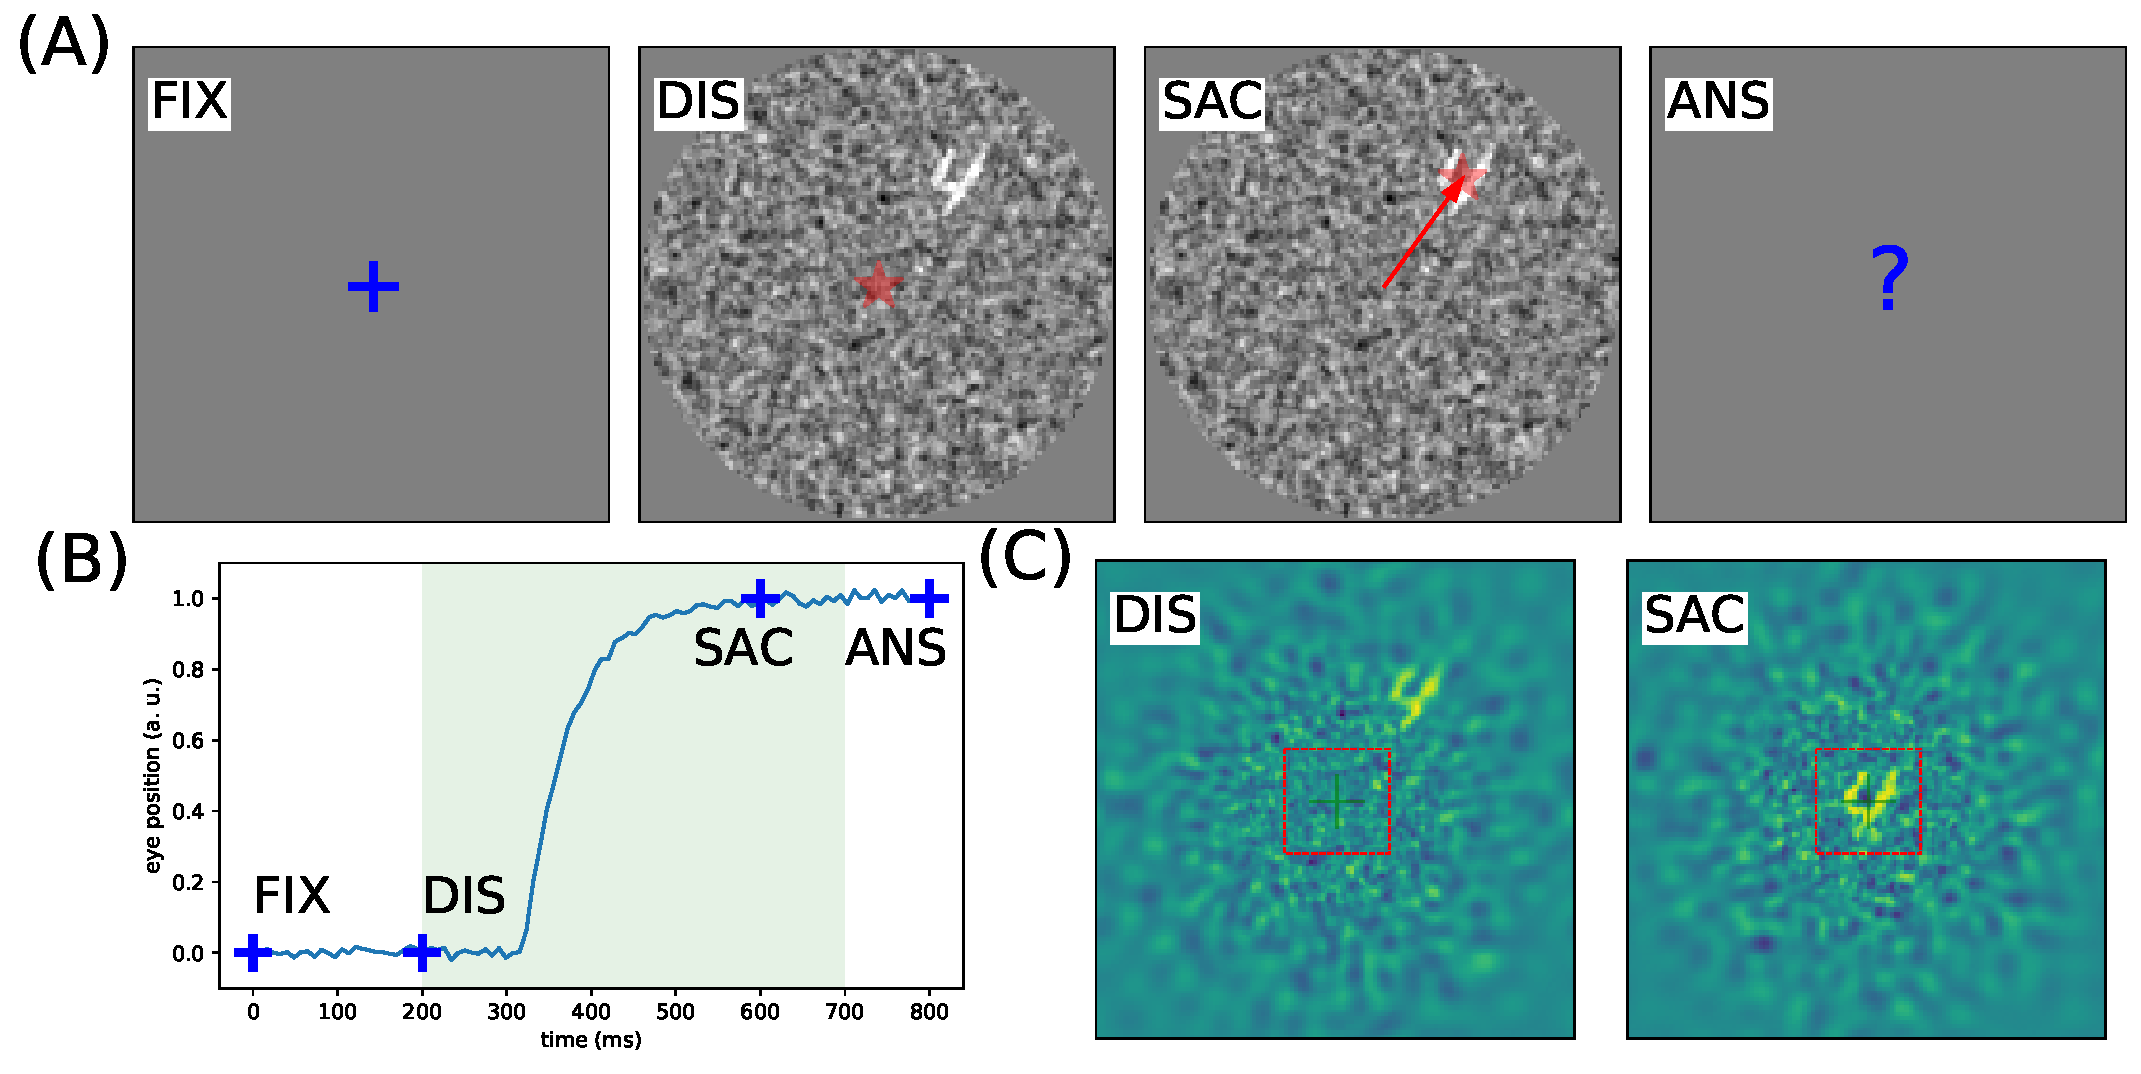
\includegraphics[width=\linewidth]{fig_intro}} %
	\caption{%
		{\bf Problem setting}: In generic, ecological settings, when searching for one target (from a class of targets) in a cluttered environment, the visual system is bound with an action selection problem. It is synthesized in the following virtual experiment: %
		\A After a fixation period \FIX\ of $200~\ms$, an observer is presented with a luminous display \DIS\ showing a single target from a known class (here digits) put at a random position within the field of view. The display is presented for a short period of $500~\ms$ (light shaded area in B), which is enough to perform at most one saccade on the potential target (\SAC , here successful). Finally, the observer has to identify the digit by a keypress \ANS. \emph{NB}: the target contrast is here enhanced to $100\%$ for better readability. %
		\B Prototypical trace of a saccadic eye movement to the target position. In particular, we show the fixation window \FIX\ and the temporal window during which a saccade is possible (green shaded area). %
		\C Simulated reconstruction of the visual information from the internal retinotopic map at the onset of the display \DIS\ and after a saccade \SAC , the dashed red box indicating the foveal region. The task does not consist in inferring the location of the target, but rather to infer an action that may provide relevant pixels at the center of fixation, allowing to identify the target's category. By comparison with the external display (see A), the action is processed from log-polar coefficients, representing a focal sample of the total visual field.
		Controlling the clutter and reducing the contrast of the digit allows to modulate the task's difficulty.
		 }%
	\label{fig:intro} %
\end{figure}%
%%------------------------------%
In contrast with phenomenological (or ``bottom-up'') approaches, active models of vision~\cite{Najemnik05,Butko2010infomax,dauce2018active} provide the ground principles of saccadic exploration. In general, they assume the existence of a generative model from which both the target position and category can be inferred through active sampling. This comes from the constraint that the visual sensor is foveated but can generate a saccade.
Several studies are relevant to our endeavor. First, one can consider optimal strategies to solve the problem of the visual search of a target~\cite{Najemnik05}. In a setting similar to that presented in Figure~\ref{fig:intro}-A, where the target is an oriented edge and the background is defined as pink noise, authors show first that a Bayesian ideal observer comes out with an optimal strategy, and second that human observers are close to that optimal performance. Though it is well predicting sequences of saccades in a perception action loop, this model is limited by the simplicity of the display (elementary edges added on stationary noise, a finite number of non-overlapping locations on a discrete grid) and by the abstract level of modeling. Despite these (inevitable) simplifications, this study could successfully predict some key characteristics of visual scanning such as the trade-off between memory content and speed. Looking more closely at neurophysiology, the study of~\cite{Samonds18} allows to go further in understanding the interplay between saccadic behavior and the statistics of the input. In this study, authors were able to manipulate the size of saccades by monitoring key properties of the presented (natural) images. For instance, smaller images generate smaller saccades. Interestingly, they also predicted the size of saccades from the size of visual receptive fields for different species, including mice which lack a foveal region. One key prediction of this study which is relevant for our problem is the fact that saccades seem optimal to \emph{a priori} decorrelate the visual input, that is, to minimize redundancy in the sequence of generated saccades, knowing the statistics of the visual inputs.

%It is one type of active inference~\cite{Friston12} (see below) and we will envision herein how to incorporate it to classical computer vision schemes.
%
A further modeling perspective is provided by~\cite{Friston12}. In this setup, a full description of the visual world is used as a generative process. An agent is completely described by the generative model governing the dynamics of its internal beliefs and is interacting with this image by scanning it through a foveated sensor, just as described in Figure~\ref{fig:intro}. Thus, equipping the agent with the ability to actively sample the visual world allows to interpret saccades as optimal experiments, by which the agent seeks to confirm predictive models of the (hidden) world. One key ingredient to this process is the (internal) representation of counterfactual predictions, that is, the probable consequences of possible hypothesis as they would be realized into actions (here, saccades). Following such an active inference scheme, numerical simulations reproduce sequences of eye movements that fit well with empirical data~\cite{Mirza18}. Compared to previous studies as~\cite{Najemnik05}, saccades are not the output of a value-based cost function such as a saliency map, but are the consequence of an active strategy by the agent to minimize the uncertainty about his beliefs, knowing his priors on the generative model of the visual world.
%
\subsection{Outline}
%
So far, few models in active vision come with an integrated processing of the visual scene, from early visual treatment toward saccade selection. The difficulty lies in combining object hypothesis (feature) space along with their spatial mapping. As pointed out earlier, the system needs to guess where the interesting objects lie in space before actually knowing what they are. Establishing the position of the objects in space is thus crucial, for it resorts to the capability of the eye to reach them with a saccade, so as to finally identify them. Inferring target's position in the peripheral visual field is thus an essential component of focal visual processing, and the acuity of such target selection ultimately conditions the capability to rapidly and efficiently process the scene. Stemming from the active vision principles, we thus address the question of the interplay of the location and identity processing in vision, and provide an artificial vision setup that efficiently implements those principles. Moreover, despite refined generative models, the processing of the visual data found in biomimetic models should resort to a combination of local features to build up posterior beliefs. Herein, our framework is made as general as possible, with minimal mathematical treatment, to speak largely to fragmented domains, such as machine learning, neuroscience and robotics.

The paper is organized as follows. After this introduction, the principles underlying accuracy-based saccadic control are defined in the second section. We first define notations, variables and equations for the generative process governing the experiment and the generative model for the active vision agent. Complex combinatorial inferences are here replaced by separate pathways, i.e. the spatial (``Where'') and categorical (``What'') pathways, whose output is combined to infer optimal eye displacements and subsequent identification of the target. Our agent, equipped with a foveated sensor, should learn an optimal behavior strategy to actively scan the visual scene. Numerical simulations are presented in the results section, demonstrating the applicability of this framework to tasks with different complexity levels. The discussion section finally summarizes the results, showing its relative advantages in comparison with other frameworks, and providing ways toward possible improvements. Implementation details are provided in the methods section, giving ways to reproduce our results, showing in particular how to simplify the learning using accuracy-driven action maps.

